\documentclass[a4paper, 11pt]{article}
\usepackage[utf8]{inputenc}
\usepackage[russian]{babel}
\usepackage{amssymb}
\usepackage{amsmath}
\usepackage{graphicx}
\usepackage{float}

\usepackage{xcolor}

\newcommand{\w}{\widetilde}

\voffset = -1cm 
\footskip=100pt
\hoffset = -1cm

\newcommand{\wide}{
\stackrel{0}{x}
}
\begin{document}
\begin{center}

\textsc{Численное моделирование нестационарного 
    одномерного течения газа с использованием схемы 
    для логарифма плотности с центральными разностями}

\end{center}

\enlargethispage{9\baselineskip}

\section{Постановка дифференциальной задачи}
Одномерное движение вязкого баротропного газа описывается системой дифференциальных уравнений:
$$
\begin{cases} 
\displaystyle{\frac{\partial \rho}{\partial t} +
 \frac{\partial \rho u}{\partial x} = f_0}, \\

\displaystyle{\rho \frac{\partial u}{\partial t} +
 \rho u \frac{\partial u}{\partial x}+ 
 \frac{\partial p}{\partial x} = 
\mu \frac{\partial^2 u}{\partial x^2}
+ \rho f}
\end{cases}
$$

\begin{center}
$
p = p (\rho)
$ - известная функция давления от плотности. 
$f_0 \equiv 0, $
$f$ - известная функция от $(t, x)$.
\end{center}
$$\mu \in [0,001; 0,1]$$

Неизвестные функции плотности и скорости:

\begin{center}
$\rho,\ u: [0, T] \times [0, X] \rightarrow \mathbb{R}$, где $T,\ X > 0$
\end{center}

$$\rho > 0$$

Краевые условия:
$$(\rho, u)|_{t=0} = (\rho_0, u_0), x \in [0, X]$$

Для гарантирования положительности $\rho$ вместо функции $\rho$ имеет смысл искать функцию $g = \ln(\rho)$ 

Тогда система дифференциальных уравнений примет вид

$$
\begin{cases}
\displaystyle{\frac{\partial g}{\partial t} + \frac{1}{2} \left(u\frac{\partial g}{\partial x} +     \frac{\partial ug}{\partial x} +(2-g)\frac{\partial u}{\partial x}\right) = f_0},\\
\displaystyle{\frac{\partial u}
{\partial t} + \frac{1}{3} \left(u 
\frac{\partial u}{\partial x} +
 \frac{\partial u^2}{\partial x}\right) +
  \tilde{p}'(g)
 \frac{\partial g}{\partial x} = \mu
  e^{-g}\frac{\partial^2 u}{\partial x^2} +
   f}
\end{cases}
$$

\section{Построение разностной схемы}
Для численного решения системы введем сетку на области $[0, T] \times [0, X]$ с шагом $h$ по оси $OX$ и $\tau$ по оси $OT$. Узел сетки с координатами $(n, m)$ соответствует точке $(n\tau, mh)$ области. Для разностных операторов и значений в узлах сетки будем использовать обозначения, введенные в пособии к вычислительному практикуму.

$M$ - количество узлов вдоль оси $OX$.
$N$ - количество узлов вдоль оси $OT$.

Запишем разностную схему:

$$
\begin{cases}
\displaystyle{G_t + \frac{1}{2}(V\hat{G}_{\wide} + (V\hat{G})_{\wide} + (2-G)V_{\wide}) = f_0},\ \ \ 1 \leqslant m \leqslant M - 1,\\
\displaystyle{G_{t,0} + \frac{1}{2} ((V\hat{G})_{x,0} + (2 - G_0)V_{x, 0})} - \\
\displaystyle{
-\frac{h}{2}((GV)_{x\overline{x}, 1} - 
\frac{1}{2}(GV)_{x\overline{x}, 2} + (2 - G_0)
(V_{x\overline{x}, 1} - 
\frac{1}{2}V_{x\overline{x}, 2})) = (f_0)_0},\\
\displaystyle{
G_{t, M} + \frac{1}{2}((V\hat{G})_{\overline{x}, M} + (2 - G_M)V_{\overline{x}, M}) +} \\ 
\displaystyle{+\frac{h}{2}((GV)_{x\overline{x}, M-1} - 
\frac{1}{2}(GV)_{x\overline{x}, M-2} + 
(2-G_M)(V_{x\overline{x}, M - 1} - 
\frac{1}{2}V_{x\overline{x}, M-2})) = (f_0)_M},\\
\displaystyle{V_t + \frac{1}{3}(V\hat{V}_{\wide} + (V\hat{V}_{\wide})) + \tilde{p}'(\hat{G})\hat{G}_{\wide} = \tilde{\mu}\hat{V}_{x\overline{x}} - 
(\tilde{\mu} - \mu e^{-\hat{G}})V_{x\overline{x}} + f},\ \ \  1 \leqslant m \leqslant M - 1,
\end{cases}
$$
где $\tilde{\mu} = \mu\vert\vert e^{-\hat{G}}\vert\vert_C$.
\\[5pt]
Запишем эту схему в следующем виде, сгруппировав слагаемые:

$$
\begin{cases}
\displaystyle{
G_{m-1}^{n+1} \left(\frac{-V_{m}^n}{2h}\right) + G_m^{n+1} \left(\frac{1}{\tau} + \frac{1}{2}\left(V_{\wide}\right)_m^n\right) +}\\
\displaystyle{ +
G_{m+1}^{n+1} \left(\frac{V_m^n}{2h}\right) + V_{m+1}^{n+1} \left(\frac{1}{2h}\right) + V_{m-1}^{n+1}\left(\frac{1}{2h}\right) =} \\
\displaystyle{
= 
f_0 (n\tau, mh) + G_m^n \left(\frac{1}{\tau} 
+\frac{1}{2} \left(V_{\wide}\right)_m^n\right)
,\ \ \  1 \leqslant m \leqslant M - 1} & (1)\\
\displaystyle{
G_0^{n+1} \left(\frac{1}{\tau} + \frac{(V_x)_0^n}{2}\right)
 + V^{n+1}_1 \left(\frac{1}{h}\right) = 
 f_0 (n\tau, 0) + \frac{G_0^n}{\tau} + } \\
 \displaystyle{ +\frac{h}{2} \left( ((GV)_{x\overline{x}})_1^n -\frac{1}{2}((GV)_{x\overline{x}})_1^n + (2 - G_0^n)((V_{x\overline{x}})_1^n - \frac{1}{2}(V_{x\overline{x}})_2^n)\right) + G_0^n \frac{(V_x)_0^n}{2} }, & (2)\\
 \displaystyle{
G_{M}^{n+1} \left(\frac{1}{\tau} + \frac{\left(V_{\overline{x}}\right)_M^n}{2}\right) + V_{M-1}^{n+1} \left(-\frac{1}{h}\right) = 
f_0(n\tau, X) + \frac{G_M^n}{\tau} + G_M^n \frac{V_{\overline{x}}}{2} - } \\
\displaystyle{
-\frac{h}{2}\left(((GV)_{x\overline{x}})_{M-1}^n
-\frac{1}{2}((GV)_{x\overline{x}})_{M-2}^n + (2-G_M^n)(V_{x\overline{x}})_{M-1}^n - 
\frac{1}{2}(V_{x\overline{x}})_{M-2}^n\right)}, & (3)\\
\displaystyle{
V_{m-1}^{n+1} \left(-\frac{V_m^n}{3h}-\left(\frac{\mu \vert\vert e^{-\hat{G}}\vert\vert_C}{h^2} \right) \right) + 
V_m^{n+1} \left(\frac{1}{\tau} + \frac{(V_{\wide})_m^n}{3} + \frac{2\mu \vert\vert e^{-\hat{G}}\vert\vert_C}{h^2}\right) +} \\
\displaystyle {
V_{m+1}^{n+1}\left(\frac{V_m^n}{3h} - 
\frac{\mu \vert\vert e^{-\hat{G}}\vert\vert_C}{h^2}\right) + G_{m-1}^{n+1}\left(-\tilde{p}'\frac{G_m^n}{2h}\right) + 
G_{m+1}^{n+1}\left(
\tilde{p}'\frac{G_m^n}{2h}\right) = } \\
\displaystyle{
 f(n\tau, mh) - (V_{x\overline{x}})_m^n \left(\mu \vert\vert e^{-\hat{G}}\vert\vert_C - \mu e^{-G_m^n} + \frac{V_m^n}{\tau}\right),\ \ \ 1 \leqslant m \leqslant M-1} & (4)
\end{cases}
$$
Будем называть \textit{$n$-ым слоем} узлы сетки с координатой по времени равной $n$.
\enlargethispage{9\baselineskip}
Заметим, что значения $V$ и $G$ известны на нулевом слое.
При известных значениях функции на слое $n$, с помощью системы уравнений, можно вычислить значения функций на $n+1$ слое. Покажем, как уравнения $(1)-(4)$ формируют необходимую СЛАУ $(*)$.

Уравнение $(1)$ для $m = 1$ и $m=M-1$ содержит четыре неизвестных, т.к. $V_0 = V_M = 0$ на любом слое. Для $2 \leqslant m \leqslant M - 2$ уравнение $(1)$ содержит пять неизвестных.\\ 
$m$, пробегая в уравнении $(1)$ значения от $1$ до $M - 1$, формирует $M-1$ уравнение в системе $(*)$ для неизвестных $G_0^{n+1}, \ldots , G_M^{n+1}$ и $V_1^{n+1}, \ldots , V_{M-1}^{n+1}$

Уравнение $(2)$ дает 1 уравнение в СЛАУ $(*)$ для неизвестных $G_0^{n+1}, V_1^{n+1}$.

Уравнение $(3)$ дает 1 уравнение в СЛАУ $(*)$ для неизвестных $G_M^{n+1}, V_{M-1}^{n+1}$.

Уравнение $(4)$ для $m =1$ и $m = M-1$ содержит четыре неизвестных, по тем же причинам, что и уравнение $(1)$, и пять при $2 \leqslant m \leqslant M - 2$.\\
$m$, пробегая в уравнении $(4)$ значения от $1$ до $M - 1$, формирует $M-1$ уравнение в системе $(*)$ для неизвестных $G_0^{n+1}, \ldots , G_M^{n+1}$ и $V_1^{n+1}, \ldots , V_{M-1}^{n+1}$

И так, СЛАУ $(*)$ является системой с $(M+1) + (M-1) = 2M$ неизвестными и $(M-1) + 1 + 1 + (M-1) = 2M$ уравнениями. В каждом уравнении не более пяти ненулевых коэффициентов.

Таким образом СЛАУ $(*)$ является разреженной, что делает естественным применение итерационных алгоритмов для ее решения.

Последовательно решая такие СЛАУ для $1 \leqslant n \leqslant N$, получим значения $G$ и $V$ во всех узлах сетки.

\section{Результаты тестовых расчетов для гладких решений}
Для проверки реализованного на ЭВМ алгоритма сделаем следующее.
\begin{enumerate}
\item Положим 
$$
\begin{cases}
\rho (t, x) = e^t (\cos (\pi x / 10) + 1.5), \\
u (t, x) = \cos (2 \pi t) \sin (\pi (x/10)^2), \\
\tilde{p}' (x) = 1.4x^{0.4}, \\
\mu =  0,01.
\end{cases}
$$
\item Аналитически вычислим $f_0$ и $f$ поставленной дифференциальной задачи с такими $\rho$ и $u$.
\item Сравним значения функций $g (t, x) = \ln (\rho (t, x))$ и $u$ в узлах сетки, вычисленные алгоритмом со значениями, вычисленными аналитически.
\end{enumerate}
Рассмотрим нормы невязок скорости и плотности на последнем слое и их динамику при изменении шага сетки.
\enlargethispage{5\baselineskip}\\

$||G_m^n - g (\tau n, hm)||_{C_h}$:
\begin{center}
\begin{tabular}{|c|c|c|c|c|}
\hline 
 N\textbackslash M &      20      &      40      &      80      &     160      \\ 
 \hline 
        20         & 3,922676e-03 & 6,846325e-03 & 7,855319e-03 & 8,028590e-03 \\ 
 \hline 
        80         & 2,284488e-03 & 6,666070e-04 & 1,385733e-03 & 1,552270e-03 \\ 
 \hline 
        320        & 3,298528e-03 & 5,208735e-04 & 1,538522e-04 & 3,205057e-04 \\ 
 \hline 
       1280        & 3,528191e-03 & 7,919148e-04 & 1,299347e-04 & 3,777771e-05 \\ 
 \hline 
\end{tabular}
\end{center}
$||G_m^n - g (\tau n, hm)||_{L2_h}$:
\begin{center}
\begin{tabular}{|c|c|c|c|c|}
\hline 
 N\textbackslash M &      20      &      40      &      80      &     160      \\ 
 \hline 
        20         & 6,978421e-03 & 8,324877e-03 & 8,596909e-03 & 8,588685e-03 \\ 
 \hline 
        80         & 2,196948e-03 & 1,066965e-03 & 1,529168e-03 & 1,638729e-03 \\ 
 \hline 
        320        & 3,151690e-03 & 4,912069e-04 & 2,865486e-04 & 3,929692e-04 \\ 
 \hline 
       1280        & 3,411053e-03 & 7,215213e-04 & 1,180613e-04 & 7,359237e-05 \\ 
 \hline 
\end{tabular}
\end{center}
$||G_m^n - g (\tau n, hm)||_{W_2^1}$:
\begin{center}
\begin{tabular}{|c|c|c|c|c|}
\hline 
 N\textbackslash M &      20      &      40      &      80      &     160      \\ 
 \hline 
        20         & 8,116420e-03 & 9,991449e-03 & 1,041680e-02 & 1,040223e-02 \\ 
 \hline 
        80         & 3,335466e-03 & 1,429192e-03 & 2,152698e-03 & 2,329049e-03 \\ 
 \hline 
        320        & 4,669536e-03 & 7,197021e-04 & 3,882380e-04 & 5,609736e-04 \\ 
 \hline 
       1280        & 5,040628e-03 & 1,078920e-03 & 1,725182e-04 & 9,975466e-05 \\ 
 \hline 
\end{tabular}
\end{center}
$||V_m^n - u (\tau n, hm)||_{C_h}$:
\begin{center}
\begin{tabular}{|c|c|c|c|c|}
\hline 
 N\textbackslash M &      20      &      40      &      80      &     160      \\ 
 \hline 
        20         & 6,536483e-03 & 7,631195e-03 & 8,045635e-03 & 8,162966e-03 \\ 
 \hline 
        80         & 3,209157e-03 & 2,053450e-03 & 2,571117e-03 & 2,735217e-03 \\ 
 \hline 
        320        & 4,584228e-03 & 6,996692e-04 & 5,508347e-04 & 6,929872e-04 \\ 
 \hline 
       1280        & 4,986150e-03 & 1,119679e-03 & 1,681524e-04 & 1,400664e-04 \\ 
 \hline 
\end{tabular}
\end{center}
$||V_m^n - u (\tau n, hm)||_{L2_h}$:
\begin{center}
\begin{tabular}{|c|c|c|c|c|}
\hline 
 N\textbackslash M &      20      &      40      &      80      &     160      \\ 
 \hline 
        20         & 1,038489e-02 & 1,248116e-02 & 1,327623e-02 & 1,348587e-02 \\ 
 \hline 
        80         & 4,157618e-03 & 3,399343e-03 & 4,243924e-03 & 4,482896e-03 \\ 
 \hline 
        320        & 5,684335e-03 & 9,515532e-04 & 9,173616e-04 & 1,137741e-03 \\ 
 \hline 
       1280        & 6,362583e-03 & 1,388733e-03 & 2,339405e-04 & 2,337295e-04 \\ 
 \hline 
\end{tabular}
\end{center}
$||V_m^n - u (\tau n, hm)||_{W_2^1}$:
\begin{center}
\begin{tabular}{|c|c|c|c|c|}
\hline 
 N\textbackslash M &      20      &      40      &      80      &     160      \\ 
 \hline 
        20         & 1,337563e-02 & 1,472665e-02 & 1,565885e-02 & 1,591049e-02 \\ 
 \hline 
        80         & 6,622063e-03 & 4,081016e-03 & 5,069747e-03 & 5,373048e-03 \\ 
 \hline 
        320        & 8,282039e-03 & 1,521293e-03 & 1,106045e-03 & 1,367516e-03 \\ 
 \hline 
       1280        & 9,028565e-03 & 2,020049e-03 & 3,772762e-04 & 2,821159e-04 \\ 
 \hline 
\end{tabular}
\end{center}

Динамикой падения невязок подтверждается сходимость решения порядка $\tau + h^2$
\enlargethispage{7\baselineskip}\\

\section{Добавление искусственной вязкости для погашения осцилляций}
Как будет видно в следующем разделе, на участках скачка или разрывов иногда возникают
осцилляции. Добавление искуственной вязкости способствует увеличению погрешности полученного решения, но так же и большей наглядности графиков в силу погашения осцилляций.

Первое уравнение схемы (2.1) изменяется следующим образом:
\\
\\
$
\displaystyle{
G_{m-1}^{n+1} \left(\frac{-V_{m}^n}{2h} \mathbin{\color{red}- \frac{\tau \eta}{h^2} (V_m^n)^2}\right) + G_m^{n+1} \left(\frac{1}{\tau} + \frac{1}{2}\left(V_{\wide}\right)_m^n \mathbin{\color{red}+ \frac{\tau \eta}{h} \left(2V_m^n (V_m^n)_{\overline{x}} + \frac{2}{h} (V_m^n)^2\right)}\right) +}\\
\displaystyle{ +
G_{m+1}^{n+1} \left(\frac{V_m^n}{2h} \mathbin{\color{red}- \frac{\tau \eta}{h}\left(2V_m^n (V_m^n)_{\overline{x}} +\frac{1}{h}(V_m^n)^2\right)}\right) + V_{m+1}^{n+1} \left(\frac{1}{2h}\right) + V_{m-1}^{n+1}\left(\frac{1}{2h}\right) =} \\
\displaystyle{
= 
f_0 (n\tau, mh) + G_m^n \left(\frac{1}{\tau} 
+\frac{1}{2} \left(V_{\wide}\right)_m^n\right)
,\ \ \  1 \leqslant m \leqslant M - 1}.
$
\\
\\

$\eta$ положим равным 1.

Для того, чтобы понять насколько велика погрешность, вносимая искусственной вязкостью,
запустим программу с конфигурацией раздела 3.
Рассмотрим нормы невязок скорости и плотности на последнем слое и их динамику при изменении шага сетки.

\newpage
$||G_m^n - g (\tau n, hm)||_{C_h}$:
\begin{center}
\begin{tabular}{|c|c|c|c|c|}
\hline 
 N\textbackslash M &      20      &      40      &      80      &     160      \\ 
 \hline 
        20         & 3,027303e-03 & 6,079820e-03 & 7,109855e-03 & 7,297630e-03 \\ 
 \hline 
        80         & 2,469829e-03 & 6,046209e-04 & 1,228040e-03 & 1,398319e-03 \\ 
 \hline 
        320        & 3,343293e-03 & 5,603700e-04 & 1,565692e-04 & 2,837960e-04 \\ 
 \hline 
       1280        & 3,539285e-03 & 8,016850e-04 & 1,392396e-04 & 4,359738e-05 \\ 
 \hline 
\end{tabular}
\end{center}
$||G_m^n - g (\tau n, hm)||_{L2_h}$:
\begin{center}
\begin{tabular}{|c|c|c|c|c|}
\hline 
 N\textbackslash M &      20      &      40      &      80      &     160      \\ 
 \hline 
        20         & 5,459609e-03 & 6,719960e-03 & 7,010482e-03 & 7,006051e-03 \\ 
 \hline 
        80         & 2,358832e-03 & 8,562423e-04 & 1,353432e-03 & 1,483715e-03 \\ 
 \hline 
        320        & 3,208420e-03 & 5,295449e-04 & 2,733631e-04 & 3,755793e-04 \\ 
 \hline 
       1280        & 3,425545e-03 & 7,323123e-04 & 1,276667e-04 & 7,330143e-05 \\ 
 \hline 
\end{tabular}
\end{center}
$||G_m^n - g (\tau n, hm)||_{W_2^1}$:
\begin{center}
\begin{tabular}{|c|c|c|c|c|}
\hline 
 N\textbackslash M &      20      &      40      &      80      &     160      \\ 
 \hline 
        20         & 6,428185e-03 & 8,471366e-03 & 9,040238e-03 & 9,082784e-03 \\ 
 \hline 
        80         & 3,448082e-03 & 1,289660e-03 & 2,093473e-03 & 2,303993e-03 \\ 
 \hline 
        320        & 4,711536e-03 & 7,339005e-04 & 3,948103e-04 & 5,730980e-04 \\ 
 \hline 
       1280        & 5,051336e-03 & 1,082671e-03 & 1,745601e-04 & 1,047004e-04 \\ 
 \hline 
\end{tabular}
\end{center}
$||V_m^n - u (\tau n, hm)||_{C_h}$:
\begin{center}
\begin{tabular}{|c|c|c|c|c|}
\hline 
 N\textbackslash M &      20      &      40      &      80      &     160      \\ 
 \hline 
        20         & 7,603278e-03 & 8,826935e-03 & 9,226537e-03 & 9,341849e-03 \\ 
 \hline 
        80         & 3,302077e-03 & 2,340227e-03 & 2,795649e-03 & 2,930461e-03 \\ 
 \hline 
        320        & 4,607151e-03 & 7,379845e-04 & 6,189833e-04 & 7,411660e-04 \\ 
 \hline 
       1280        & 4,991859e-03 & 1,125517e-03 & 1,803059e-04 & 1,568410e-04 \\ 
 \hline 
\end{tabular}
\end{center}
$||V_m^n - u (\tau n, hm)||_{L2_h}$:
\begin{center}
\begin{tabular}{|c|c|c|c|c|}
\hline 
 N\textbackslash M &      20      &      40      &      80      &     160      \\ 
 \hline 
        20         & 1,169881e-02 & 1,380130e-02 & 1,455186e-02 & 1,474642e-02 \\ 
 \hline 
        80         & 4,310347e-03 & 3,716146e-03 & 4,506701e-03 & 4,728942e-03 \\ 
 \hline 
        320        & 5,673148e-03 & 1,013637e-03 & 9,924577e-04 & 1,198472e-03 \\ 
 \hline 
       1280        & 6,357793e-03 & 1,389623e-03 & 2,519741e-04 & 2,521522e-04 \\ 
 \hline 
\end{tabular}
\end{center}
$||V_m^n - u (\tau n, hm)||_{W_2^1}$:
\begin{center}
\begin{tabular}{|c|c|c|c|c|}
\hline 
 N\textbackslash M &      20      &      40      &      80      &     160      \\ 
 \hline 
        20         & 1,535277e-02 & 1,660978e-02 & 1,742239e-02 & 1,763747e-02 \\ 
 \hline 
        80         & 6,948748e-03 & 4,541354e-03 & 5,394857e-03 & 5,659660e-03 \\ 
 \hline 
        320        & 8,309691e-03 & 1,638142e-03 & 1,212322e-03 & 1,438737e-03 \\ 
 \hline 
       1280        & 9,032652e-03 & 2,033500e-03 & 4,099248e-04 & 3,079729e-04 \\ 
 \hline 
\end{tabular}
\end{center}

\section{Результаты расчетов для негладких начальных данных}
Решим 2 задачи с негладкими начальными данными.
\begin{equation}
\begin{split}
& f_0 \equiv  0, \\
& f_1  \equiv 0, \\
& \tilde{p}' (x) = 1.4x^{0.4}
\end{split}
\end{equation}

$$
(1)\quad \quad
\begin{cases}
\rho_0(x) = 1, \quad x < 4,5 \text{ или } x > 5,5,\\
\rho_0(x) = 2, \quad x \in [4,5; 5,5],\\
u_0(x) \equiv 0, \quad x \in [0; 10],\\
u(t, 0) = u(t, 10) = 0, \quad t \in [0; 1], \\
& \mu =  0,01, \\
\end{cases}
$$

$$
(2)\quad \quad
\begin{cases}
u_0(x) = 0, \quad x < 4,5 \text{ или } x > 5,5,\\
u_0(x) = 1, \quad x \in [4,5; 5,5],\\
\rho_0(x) \equiv 1, \quad x \in [0; 10],\\
u(t, 0) = u(t, 10) = 0, \quad t \in [0; T],\\
& \mu =  0,1. \\
\end{cases}
$$
Настройки алгоритма:
$$
M = 600,
N = 600.
$$
Для задачи (1) \textit{без добавления искусственной вязкости} получаем:
\begin{figure}[H]
	\begin{minipage}[H] {0.49\linewidth}
		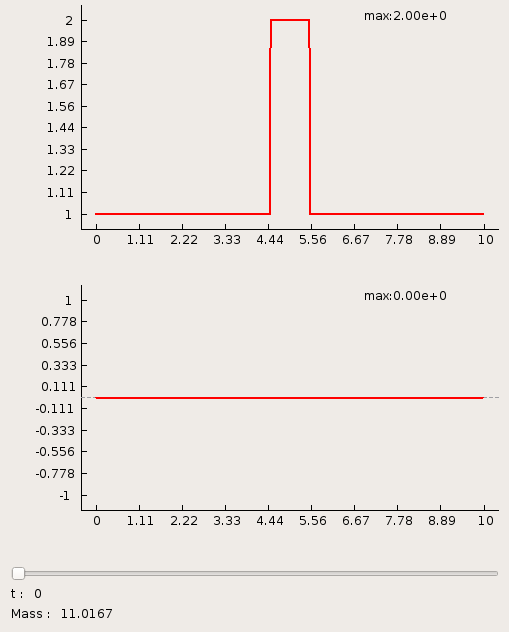
\includegraphics[width=1\linewidth]{p1/p1_t=0.png}
	\end{minipage}%
	\begin{minipage}[H] {0.49\linewidth}
		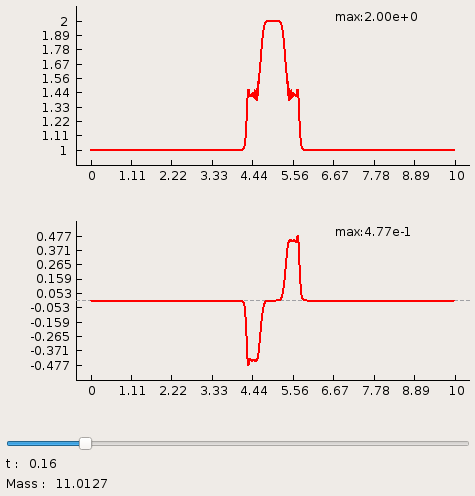
\includegraphics[width=1\linewidth]{p1/p1_t=0,16.png}
	\end{minipage}
\end{figure}
\newpage
\begin{figure}[h]
	\begin{minipage}[H] {0.49\linewidth}
		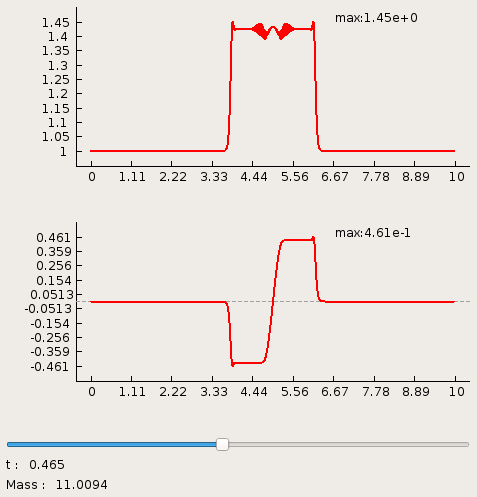
\includegraphics[width=1\linewidth]{p1/p1_t=0,465.png}
	\end{minipage}%
		\begin{minipage}[H] {0.49\linewidth}
		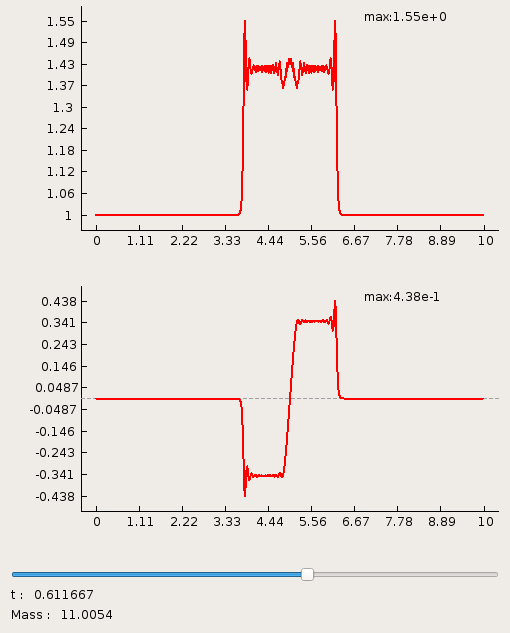
\includegraphics[width=1\linewidth]{p1/p1_t=0,611.png}
	\end{minipage}
%	\end{figure}
%\begin{figure}[H]
	\begin{minipage}[H] {0.49\linewidth}
		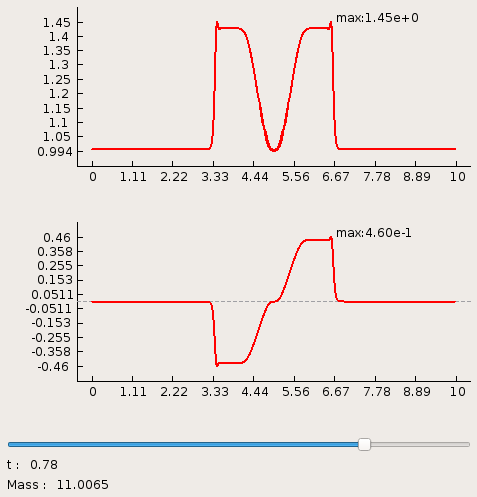
\includegraphics[width=1\linewidth]{p1/p1_t=0,78.png}
	\end{minipage}
	\begin{minipage}[H] {0.49\linewidth}
		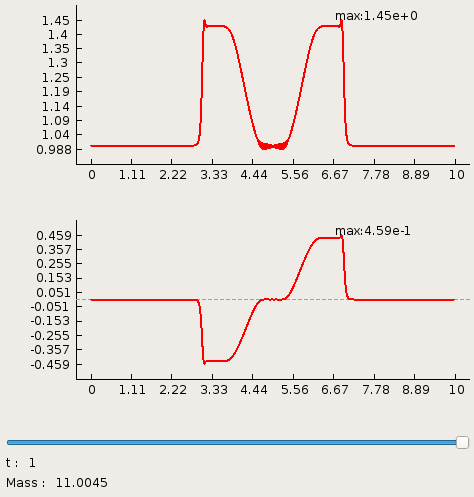
\includegraphics[width=1\linewidth]{p1/p1_t=1.png}
	\end{minipage}
	\caption{Графики плотности (верхний) и скорости (нижний)}
\end{figure}

Для задачи (1) \textit{с добавлением искусственной вязкости} получаем
\begin{figure}[H]
	\begin{minipage}[H] {0.49\linewidth}
		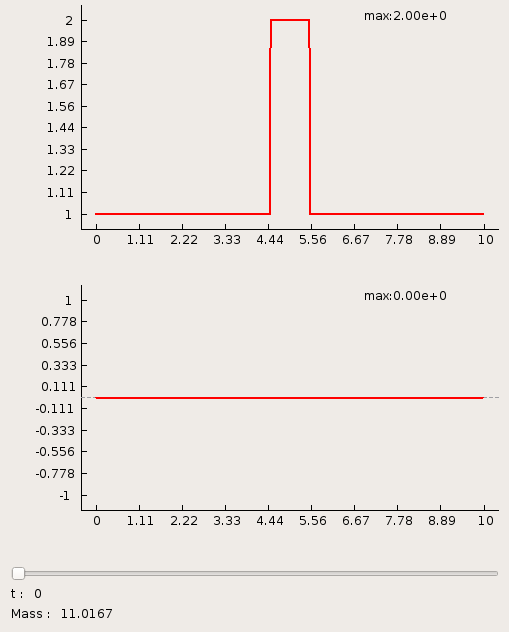
\includegraphics[width=1\linewidth]{p1/p1_t=0.png}
	\end{minipage}
	\begin{minipage}[H] {0.49\linewidth}
		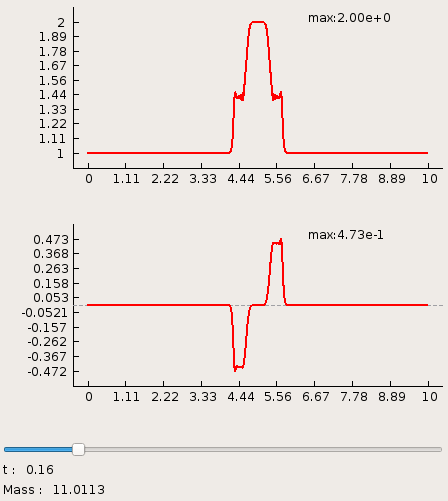
\includegraphics[width=1\linewidth]{p1/p1_t=0,16_supr.png}
	\end{minipage}
	\begin{minipage}[H] {0.49\linewidth}
		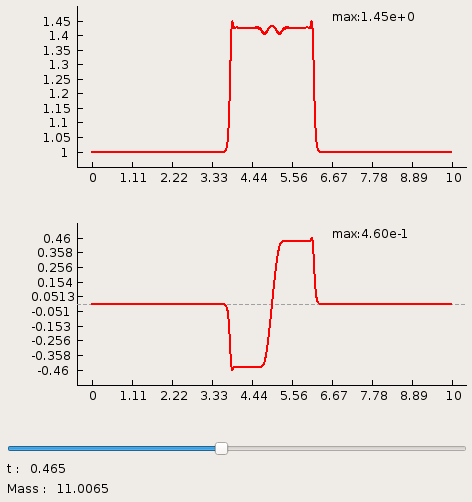
\includegraphics[width=1\linewidth]{p1/p1_t=0,465_supr.png}
	\end{minipage}
		\begin{minipage}[H] {0.49\linewidth}
		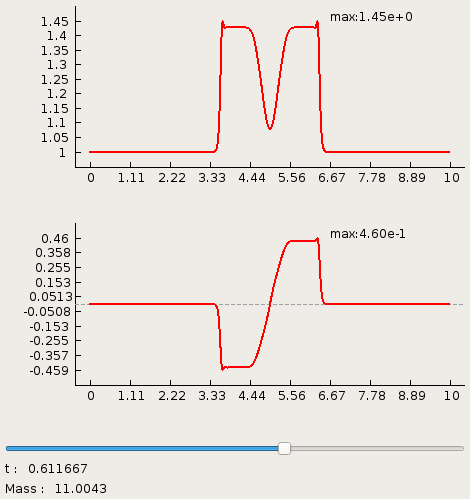
\includegraphics[width=1\linewidth]{p1/p1_t=0,611_supr.png}
	\end{minipage}
	\end{figure}
\begin{figure}[H]
	\begin{minipage}[H] {0.49\linewidth}
		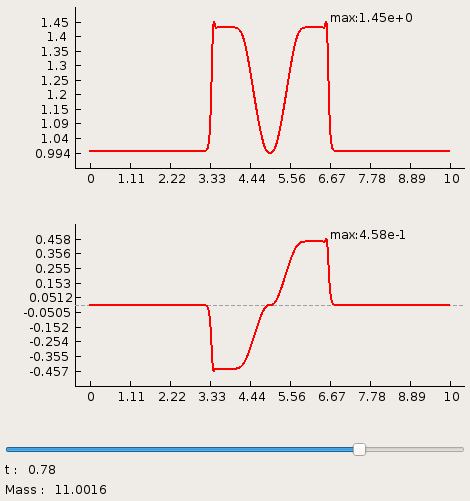
\includegraphics[width=1\linewidth]{p1/p1_t=0,78_supr.png}
	\end{minipage}
	\begin{minipage}[H] {0.49\linewidth}
		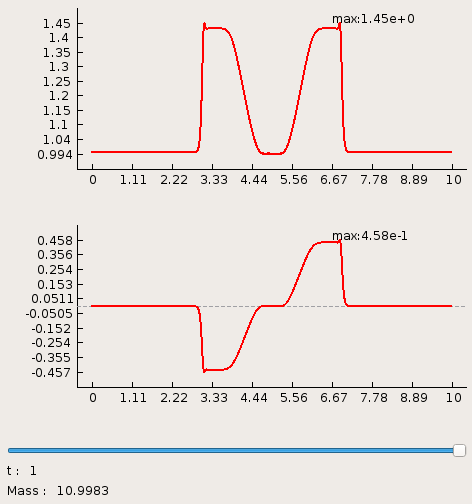
\includegraphics[width=1\linewidth]{p1/p1_t=1_supr.png}
	\end{minipage}
	\caption{Графики плотности (верхний) и скорости (нижний)}
\end{figure}
Заметим, что закон сохранения масс выполнен, т.к. изменяется в пределах вычислительной погрешности.

Для задачи (2) \textit{без добавления искусственной вязкости} получаем:
\begin{figure}[H]
	\begin{minipage}[h] {0.49\linewidth}
		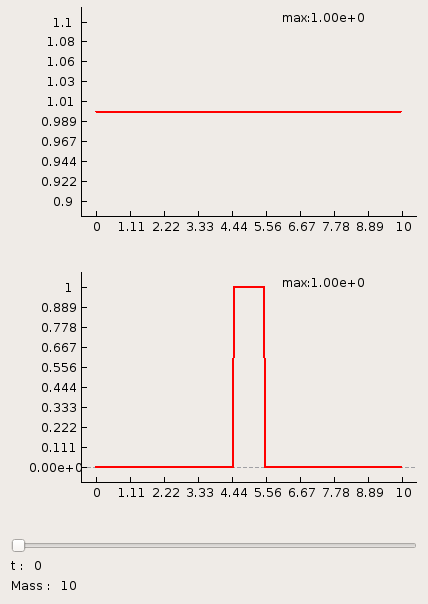
\includegraphics[width=1\linewidth]{p2/p2_t=0.png}
	\end{minipage}
	\begin{minipage}[h] {0.49\linewidth}
		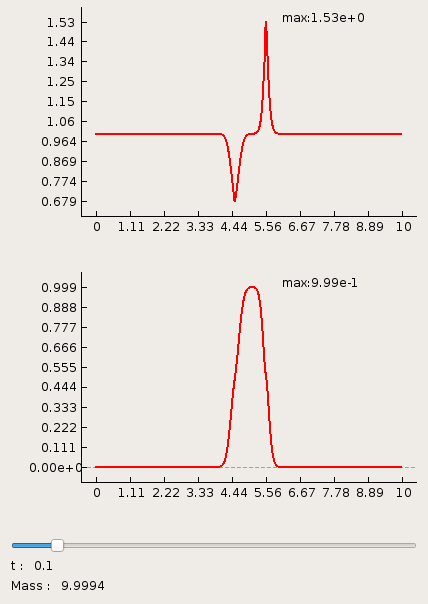
\includegraphics[width=1\linewidth]{p2/p2_t=0,1.png}
	\end{minipage}
\end{figure}
\begin{figure}[H]
	\begin{minipage}[h] {0.49\linewidth}
		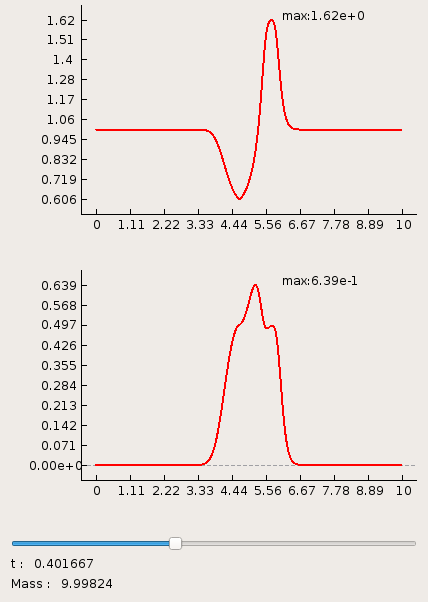
\includegraphics[width=1\linewidth]{p2/p2_t=0,4.png}
	\end{minipage}
		\begin{minipage}[h] {0.49\linewidth}
		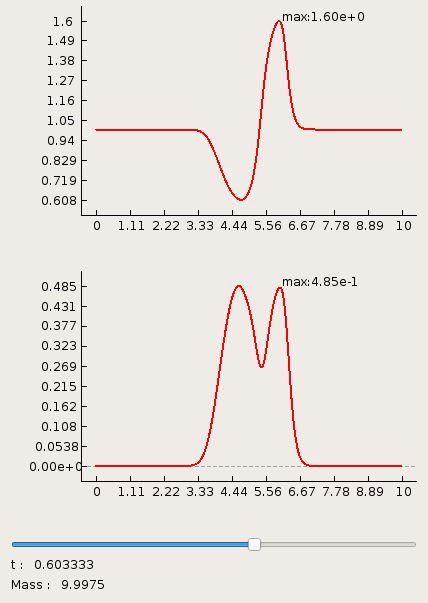
\includegraphics[width=1\linewidth]{p2/p2_t=0,6.png}
	\end{minipage}

	\begin{minipage}[h] {0.49\linewidth}
		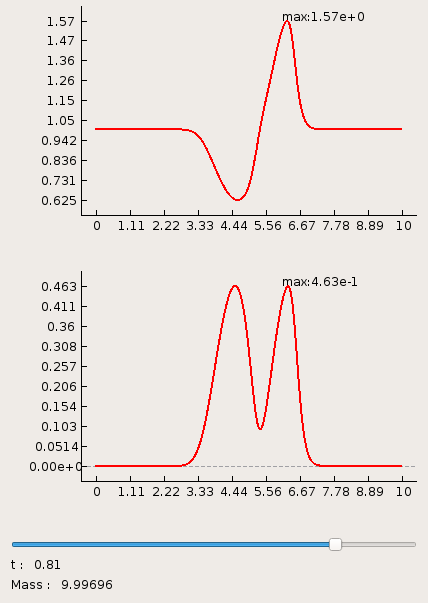
\includegraphics[width=1\linewidth]{p2/p2_t=0,8.png}
	\end{minipage}
	\begin{minipage}[h] {0.49\linewidth}
		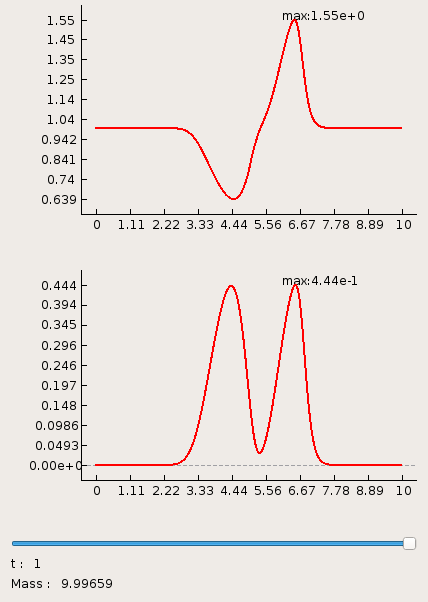
\includegraphics[width=1\linewidth]{p2/p2_t=1.png}
	\end{minipage}
	\caption{Графики плотности (верхний) и скорости (нижний)}
\end{figure}


Закон сохранения массы так же выполнен.

\section{Зависимость точности полученного решения от коэффициента вязкости газа}
Для задачи 4.1 проведем три запуска программы с
$$
\begin{cases}
 f_0 \equiv  0, \\
 f_1  \equiv 0, \\
 \tilde{p}'(z) = 1.4z^{0.4}, \\
M = 800, \\
 N = 800, \\
 \mu \in \{0.001, 0,01, 0.1\}
\end{cases}
$$
Имеем следующую зависимость точности полученного решения от коэффициента вязкости газа:

\begin{tabular}{|l|c|c|c|}
\hline
норма $\backslash \ \mu$ 					& 0.001      & 0.01       & 0.1 \\
\hline
$\|G_m^n - g (\tau n, hm)|_{C_h}$ 			& 2,584176e-04 & 3,700739e-04 & 2,817834e-03 \\
\hline
$\|G_m^n - g (\tau n, hm)|_{L_{2,h}}$ 		& 3,207805e-04 & 4,151149e-04 & 2,019011e-03 \\
\hline
$\|G_m^n - g (\tau n, hm)|_2^1$ 			& 5,062162e-04 & 7,514924e-04 & 5,873506e-03 \\
\hline
$\|V_m^n - u (\tau n, hm)|_{C_h}$ 			& 4,216830e-04 & 4,278619e-04 & 2,062970e-03 \\
\hline
$\|V_m^n - u (\tau n, hm)|_{L_{2,h}}$ 		& 6,341970e-04 & 6,255225e-04 & 1,524787e-03 \\
\hline
$\|V_m^n - u (\tau n, hm)|_2^1$ 			& 7,866074e-04 & 8,754409e-04 & 5,837614e-03 \\
\hline
\end{tabular}\\

\section{Стабилизация газа на негладких начальных условиях}
Интересно построить решение разностной схемы на области, неограниченной по времени. Вместо этого критерием окончания итеративного процесса, может являться достаточно малая разность между максимальным и минимальным значением плотности газа на $[0, X]$. Приведем графические результаты работы алгоритма на задаче (4.1) с критерием для плотности $\varepsilon = 10^-2$.
Запустим программу \textit{без добавления искусственной вязкости} со следующими параметрами:
$$
\begin{cases}
 f_0 \equiv  0, \\
 f_1  \equiv 0, \\
 \tilde{p}'(z) = 1.4z^{0.4}, \\
 h = 0.125, \\
 \tau = 0.125, \\
 \mu = 0.1
\end{cases}
$$
\begin{figure}[H]
	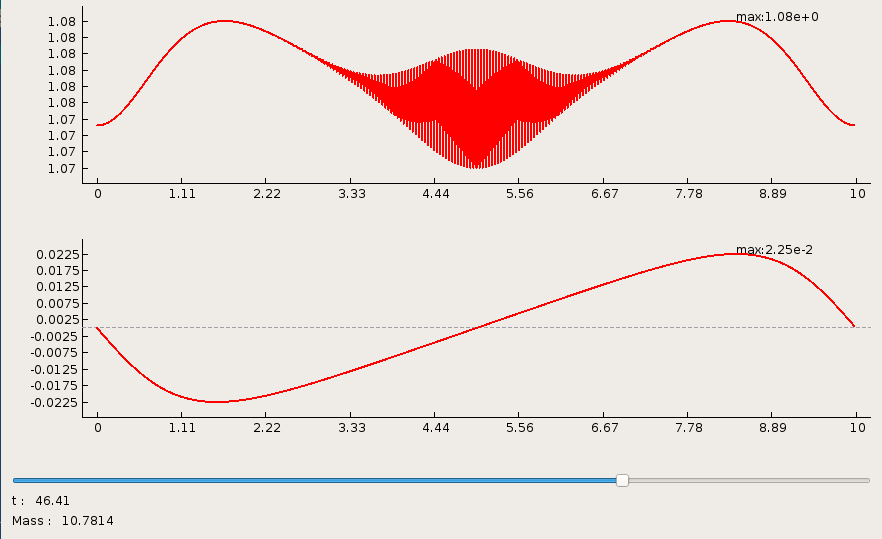
\includegraphics[width=1\linewidth]{p3/p3_rho_t=46,41.png}
\end{figure}

Запустим программу \textit{c добавлением искусственной вязкости} со теми же параметрами
\begin{figure}[H]
	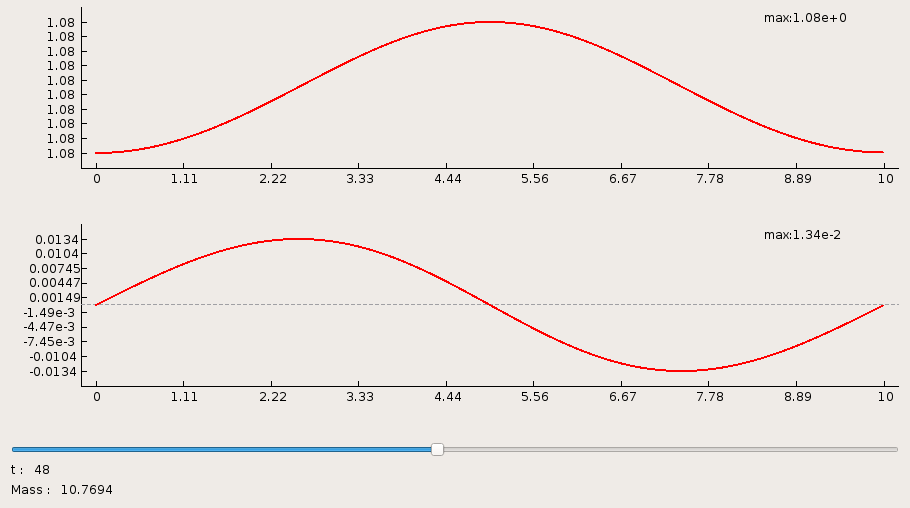
\includegraphics[width=1\linewidth]{p3/p3_t=48_noscill.png}
\end{figure}
\end{document}
